% Layout: (_5,_4):(_8,_2)
\documentclass[convert]{standalone}
\usepackage{tikz}

\begin{document}
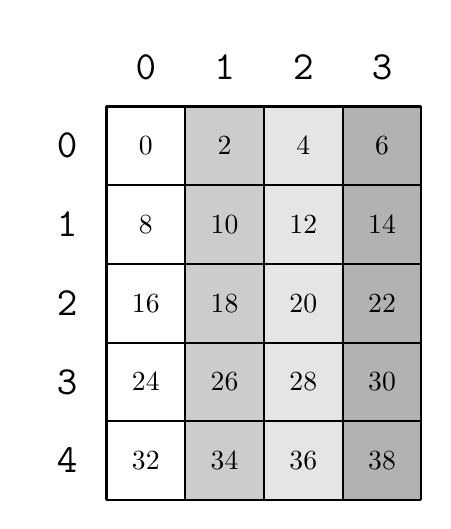
\begin{tikzpicture}[x={(0cm,-1cm)},y={(1cm,0cm)},every node/.style={minimum size=1cm, outer sep=0pt}]

\node[fill=black!00] at (0,0) {0};
\node[fill=black!20] at (0,1) {2};
\node[fill=black!10] at (0,2) {4};
\node[fill=black!30] at (0,3) {6};
\node[fill=black!00] at (1,0) {8};
\node[fill=black!20] at (1,1) {10};
\node[fill=black!10] at (1,2) {12};
\node[fill=black!30] at (1,3) {14};
\node[fill=black!00] at (2,0) {16};
\node[fill=black!20] at (2,1) {18};
\node[fill=black!10] at (2,2) {20};
\node[fill=black!30] at (2,3) {22};
\node[fill=black!00] at (3,0) {24};
\node[fill=black!20] at (3,1) {26};
\node[fill=black!10] at (3,2) {28};
\node[fill=black!30] at (3,3) {30};
\node[fill=black!00] at (4,0) {32};
\node[fill=black!20] at (4,1) {34};
\node[fill=black!10] at (4,2) {36};
\node[fill=black!30] at (4,3) {38};
\draw[color=black,thick,shift={(-0.5,-0.5)}] (0,0) grid (5,4);

\node at (0,-1) {\Large{\texttt{0}}};
\node at (1,-1) {\Large{\texttt{1}}};
\node at (2,-1) {\Large{\texttt{2}}};
\node at (3,-1) {\Large{\texttt{3}}};
\node at (4,-1) {\Large{\texttt{4}}};
\node at (-1,0) {\Large{\texttt{0}}};
\node at (-1,1) {\Large{\texttt{1}}};
\node at (-1,2) {\Large{\texttt{2}}};
\node at (-1,3) {\Large{\texttt{3}}};
\end{tikzpicture}
\end{document}
